Bei Angular handelt es sich um eines der beliebtesten JavaScript-Web-Frameworks am Markt. Angular gibt es bereits seit 2009, seitdem treibt das Entwicklerteam das Ziel an ein Framework zu erschaffen, welches sowohl die Endbenutzer:innen, als auch die Entwickler:innen gerne verwenden. Durch diese Grundsätze entstand im Laufe der Zeit eine riesige Community. Ein großer Meilenstein ist das Jahr 2016, in dem das Web-Framework komplett in Typescript umgeschrieben wurde.

\begin{figure}[h!]
    \centering
    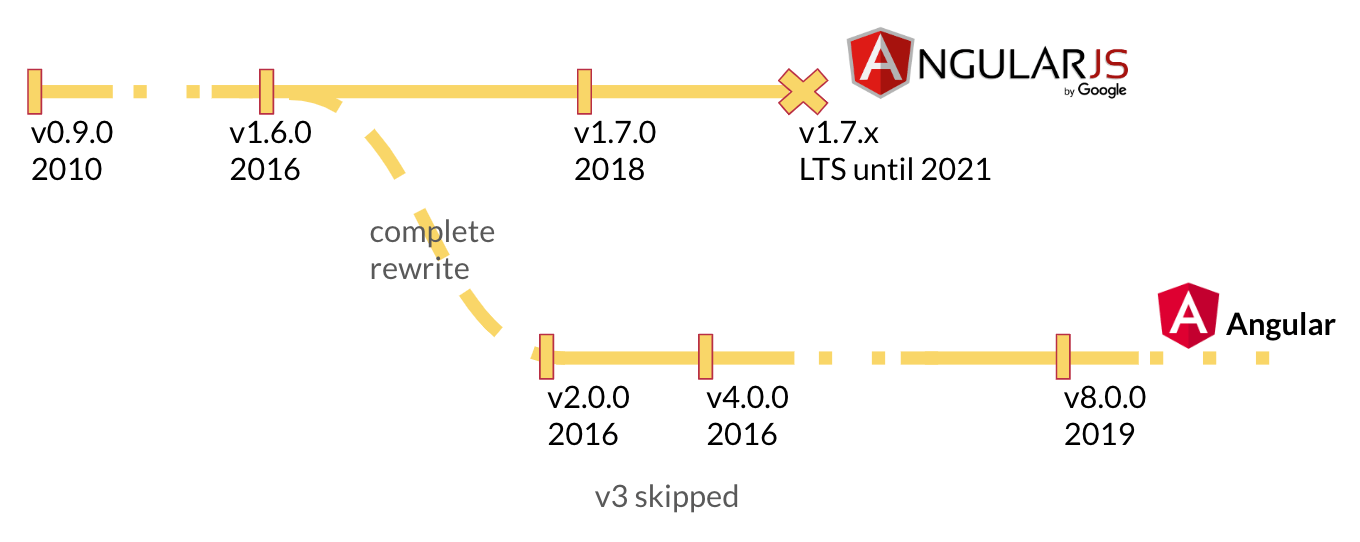
\includegraphics[width=1\textwidth]{pics/angular-versions.png}
    \caption{Angular Versionen}
    \cite{frontend_web_angular_introduction}
    \label{fig:mesh1}
\end{figure}

Früher sorgte diese Veränderung für viel Aufregen, heute ist dies jedoch anders, da die Verwendung von Typescript immer mehr zum Standard geworden ist.

\subsubsection{Aufbau}
Angular hat ein sehr großes System, welches folgendermassen aufgebaut ist:

\begin{figure}[h!]
    \centering
    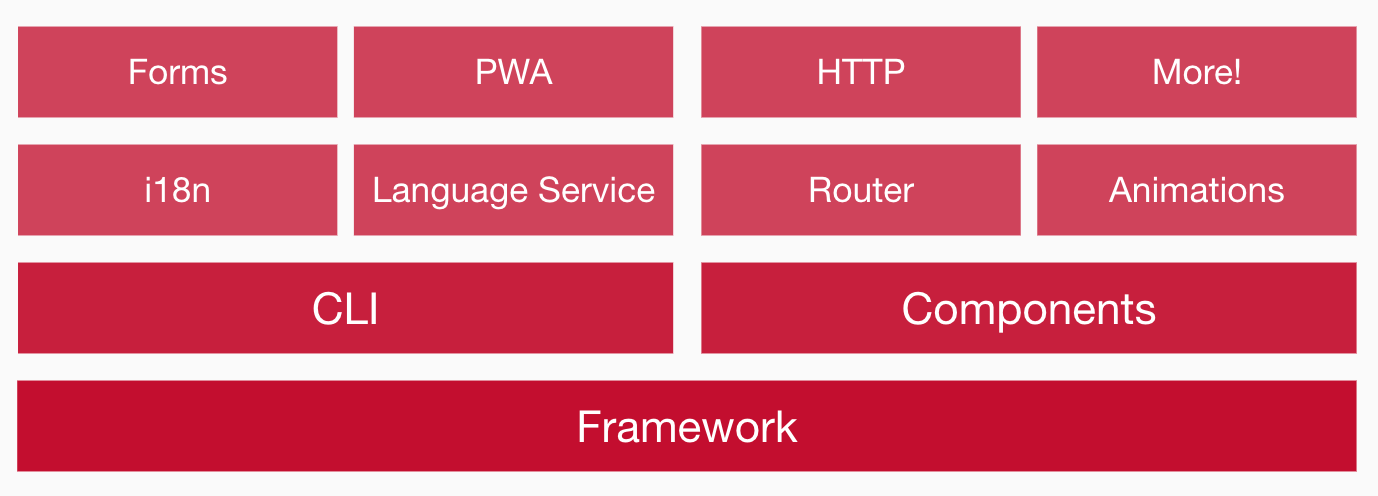
\includegraphics[width=1\textwidth]{pics/angular-architecture.png}
    \caption{Angular Aufbau}
    \cite{frontend_web_angular_introduction}
    \label{fig:mesh1}
\end{figure}

Grundlegend gibt es das sogenannte Core-Framework, wo die allgemeinen Konzepte festgelegt sind. Des weiteren gibt es noch zwei weitere wichtige Konzepte. Das sind die Angular CLI und die Verwaltung der jeweiligen Komponenten. Dieser Aufbau ist in ziemlich jeden Projekt enthalten und bietet die Grundfunktionalität, die Angular mit sich bringt. Zusätzlich gibt es noch zahlreiche weitere Module, welche zwar optional sind, jedoch in den meisten Fällen verwendet werden. Hier sind die bekanntesten Beispiele:

\begin{itemize}
    \item Routing  (Routing für Single Page Applications)
    \item forms (Formulare und Validierung)
    \item i18n (Mehrsprachige Anwendungen)
    \item Animations (Animationen für Transitionen)
    \item PWA  (Offline Funktionalität)
    \item HTTP (HTTP, Rest und GraphQL Kommunikation)
\end{itemize}

\subsubsection{Installation}
Für die Installation von Angular wird \textbf{npm} benötigt.

\begin{lstlisting}
    npm i -g @angular/cli
\end{lstlisting}

Mit diesem Command Line Befehl kann man die Angular CLI global installieren. Nach dieser Installation kann man den \textbf{ng} Befehl verwenden. Um alle Möglichkeiten davon zu sehen gibt es folgenden Befehl:

\begin{lstlisting}
    ng --help
\end{lstlisting}
\newline
\begin{lstlisting}
    ng new angular-diplomarbeit
\end{lstlisting}

Mit \textbf{ng new} kann man ein neues Projekt mit einem benutzerdefinierten Namen erstellen. Man wird dann gefragt ob man das Angular Routing Module bereits vorinstalliert hat und welche Art von Stylesheet man verwenden möchte. Zusätzlich kann man noch entscheiden ob die Daten des Projektes anonym geteilt werden dürfen. Dies hilft dem Entwicklerteam von Angular das Framework anhand von reelen Daten ständig zu verbessern. Wenn das Projekt erfolgreich angelegt wurde kann man dieses mit dem Befehl \textbf{ng serve} lokal starten.

\begin{lstlisting}
    ng serve
\end{lstlisting}

Standardmäßig ist dieses Projekt unter http://localhost:4200 im Browser erreichbar. 

\subsubsection{Komponenten}
Angular verwendet, ähnlich wie andere beliebte Frameworks, Komponenten. Diese bilden die einzelnen Bausteine für eine Anwendung.

\begin{figure}[h!]
    \centering
    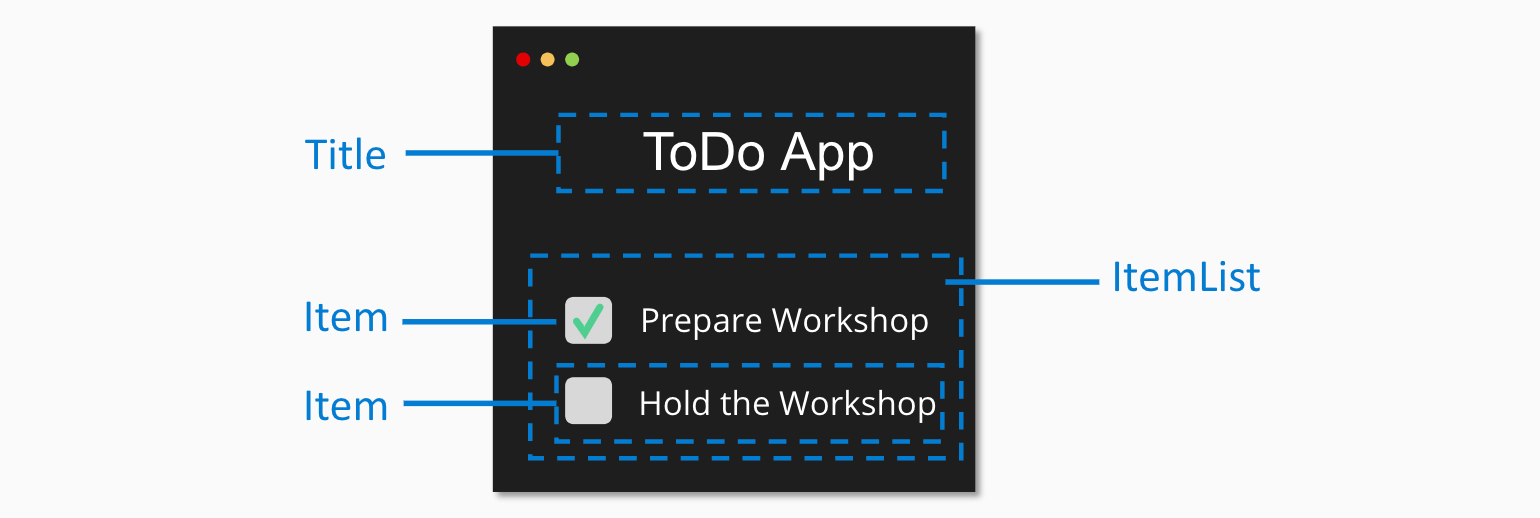
\includegraphics[width=1\textwidth]{pics/angular-components.png }
    \caption{Angular Aufbau}
    \cite{frontend_web_angular_introduction}
    \label{fig:mesh1}
\end{figure}

In diesem Beispiel sieht man wie eine sinnvolle Aufteilung einer Benutzeroberfläche in Komponenten aussehen könnte. Hierbei gibt es zunächst den Title, dieser steht als eigener Teil da und sollte somit als eigene Komponente ausgelagert werden. Des weiteren gibt es eine Liste von Items. Hierbei gibt es zunächst eine Komponente für die Liste und in dieser sind dann mehrere Items, welche wiederum jeweils eigene Komponenten sind. 

Die Einbindung solcher Komponenten in HTML könnte in Angular folgendermassen aussehen:

\begin{lstlisting}[caption=Angular Komponenten Einbindung]
    <todo-title>ToDo App</todo-title>
    <todo-list>
      <todo-item state="checked">Prepare Workshop</todo-item>
      <todo-item>Hold the Workshop</todo-item>
    </todo-list>
\end{lstlisting}

Die Logik von Komponenten ist mit Typescript realisiert, dass ermöglicht im Vergleich zu standardmäßigen JavaScript einige Vorteile. Der größte Unterschied ist die Typisierung, welche in JavaScript nicht wirklich vorhanden ist. Damit ist eine Anwendung weniger fehleranfällig und der Code ist sauberer und klarer strukturiert. Zusätzlich bietet Typescript jedoch auch noch die Verwendung von \textbf{Decorators}. Darunter versteht man strukturierte Metadaten, welche einer Klasse zugewiesen werden.

\newpage

Es gibt vier Bestandteile, welche eine Angular Komponente ausweist:

\begin{itemize}
    \item Decorator (macht die Komponente im Projekt “bekannt”)
    \item Selektor (definiert das HTML Element welches erzeugt wird)
    \item HTML-Template (für die Darstellung)
    \item Klasse (beinhaltet Interface und Logik)
\end{itemize}

Erstellt wird eine Angular Komponente mit folgendem Befehl:

\begin{lstlisting}
    ng generate component info-box
\end{lstlisting}

In diesem Beispiel wird eine Komponente für eine Infobox erstellt, dafür werden vier neue Files generiert und die Komponente automatisch im Projekt definiert.

\begin{lstlisting}[caption=Komponentenerstellung Konsolenausgabe]
    CREATE src/app/info-box/info-box.component.scss (0 bytes)
    CREATE src/app/info-box/info-box.component.html (23 bytes)
    CREATE src/app/info-box/info-box.component.spec.ts (636 bytes)
    CREATE src/app/info-box/info-box.component.ts (277 bytes)
    UPDATE src/app/app.module.ts (0 bytes)
\end{lstlisting}

Das ist der Konsolen Output, der beim Erstellen einer Komponente ausgegeben wird. Es ist erkennbar, dass ein Ordner erstellt wird mit vier Dateien. Ebenfalls wird die Komponente in \textbf{app.module.ts} registriert. Das ist wichtig damit dieses im ganzen Projekt erkannt und eingebunden werden kann.

Für die Programmierer:innen sind jedoch eigentlich nur zwei Dateien relevant.
Die erste ist \textbf{info-box.component.ts}, diese sieht wie folgt aus:

\begin{lstlisting}[caption=Angular Typescript Komponente Grundaufbau]
    @Component({
      selector: "app-info-box",
      templateUrl: "./info-box.component.html",
      styleUrls: ["./info-box.component.scss"],
    })
    export class InfoBoxComponent implements OnInit {
      constructor() {}
    
      ngOnInit() {}
    }
\end{lstlisting}

Dabei sind zu erst einige grundlegende Informationen definiert, wie Abhängigkeiten und der Selektor-Name. Das ist der Name mit dem die Komponente eingebunden werden kann.

\begin{lstlisting}
    <app-info-box></app-info-box>
\end{lstlisting}

Die zweite wichtige Datei ist die \textbf{info-box.component.html}, in welcher der HTML-Code definiert wird.

\subsubsection{Services}
Die Logik für eine Anwendung muss nicht unbedingt in den jeweiligen Komponenten definiert sein, sondern kann in einen Angular Service ausgelagert werden. Diese kann dann von mehreren Komponenten benutzt werden und bietet eine bessere Übersicht für die Programmierer:innen.
Ebenfalls können in einem Service Daten gespeichert werden, welche dann von mehreren Komponenten verwendet oder geändert werden können.

\subsubsection{Expressions}
Damit eine Komponente nicht nur aus statischen Inhalten besteht, stellt Angular Expressions zur Verfügung.
Expression Syntax:

\begin{lstlisting}
    {{ expression }}
\end{lstlisting}

Hier ist ein Beispiel für die Verwendung einer Expression in einer Komponente:

\begin{lstlisting}[caption=Expression Verwendung]
    class TestComponent implements OnInit {
      text = "HTL Leonding Diplomarbeit";
    
      constructor() {}
    
      ngOnInit() {}
    }
\end{lstlisting}

In einer Komponente wird eine Variable namens \textbf{text} definiert. Diese kann folgendermassen in HTML eingebunden werden:

\begin{lstlisting}
    <p>{{ text }}</p>
\end{lstlisting}

Wenn sich der Wert dieser Variable nun verändert, wird diese gleichzeitig auch auf der Benutzerfläche aktualisiert. 

\subsubsection{Property Binding}
Damit verbindet Angular TypeScript Properties direkt mit der Logik von HTML. Hier ein Beispiel:

\begin{lstlisting}[caption=Angular Variablen Initalisierung]
    class TestComponent implements OnInit {
      text = "HTL Leonding Diplomarbeit";
      hidden = true;
    
      constructor() {}
    
      ngOnInit() {}
    }
\end{lstlisting}

Es wurde zusätzlich eine Variable namens \textbf{hidden} erstellt, welche einen Boolean mit dem Wert \textbf{true} darstellt.

\begin{lstlisting}
    <p [hidden]="hidden">{{ text }}</p>
\end{lstlisting}

Solange diese Variable nun auf \textbf{true} gesetzt ist wird das HTML Element versteckt.

\subsubsection{Event Binding}
Des weiteren gibt es noch das sogenannte Event Binding. Damit können verschiedene Events auf der Benutzerfläche abgefangen und mit der Logik von Angular verbunden werden.

\begin{lstlisting}
    <button (click)="hidden=!hidden">Text ein-/ausblenden</button>
    <p [hidden]="hidden">{{ text }}</p>
\end{lstlisting}

In diesem Beispiel wird die hidden Variable beim Klicken eines Buttons geändert und somit der Text jeweils ein- oder ausgeblendet.

\subsubsection{Schleifen}
Ebenfalls kann man in HTML Schleifen definieren. Dafür wird, wie in folgenden Beispiel, ngFor verwendet.
Zuerst braucht man dafür eine Variable, welche ein Array ist.

\begin{lstlisting}[caption=Typescript Array]
    tasks = [
      {
        title: "Diplomarbeit schreiben",
      },
      {
        title: "Diplomarbeit korrigieren",
      },
      {
        title: "Diplomarbeit abgeben",
      },
    ];
\end{lstlisting}

Diese Variable kann im HTML-Code durchiteriert werden:

\begin{lstlisting}[caption=Angular Schleife]
    <ul>
      <li *ngFor="let task of tasks">
        <span>{{task.title}}</span>
      </li>
    </ul>
\end{lstlisting}

\cite{frontend_web_angular_introduction}


